\section{Project: Speech emotion recognition for edge devices}
\subsection{Motivation}
Human vocal language is an interesting topic that has inspired researchers to explore speech communication with machines for a long time. Various applications, such as smartphone assistants, speech-to-text converters, and voice-operated machines, have been developed in this domain.
However, catching up with human speech is not enough. By enabling machines to recognize and understand human emotions, we can enhance their ability to comprehend us more effectively.

Speech emotion recognition (SER) is a subfield of speech recognition that aims to classify a human speaker's emotional state. It is vital in this domain as it empowers machines to identify and respond to human emotions. Its applications span multiple fields, including safety, entertainment, and biomedicine. 
An exemplary use case is automatic call assistance systems, where understanding customer emotions is vital for providing appropriate service. By discerning emotions, such systems can redirect calls from angry or dissatisfied customers to human agents, ensuring personalized assistance.
In web-based movies and computer tutorials, SER can enhance the viewer's experience by adapting content based on their emotional state [25]

\begin{center}
    \begin{figure}[!htp]
        \centering
        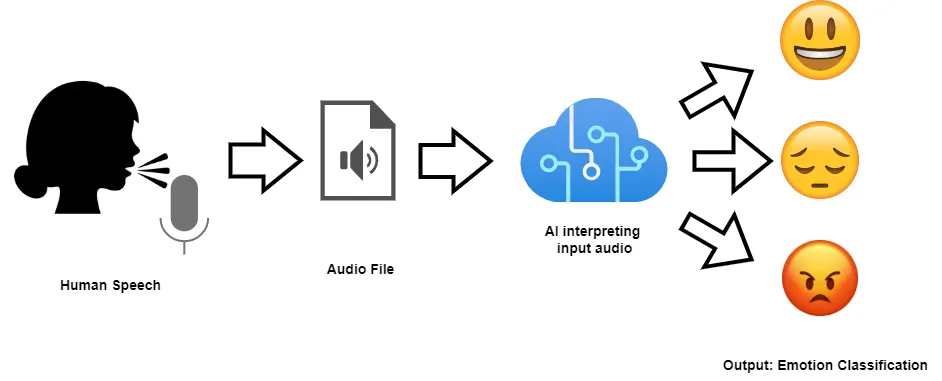
\includegraphics[width=0.8 \textwidth]{image/speech_recognition}
        \caption{Speech recognition system}
        \label{subsection}
    \end{figure}
    \end{center}

In the automotive industry, SER can serve as a safety feature. By monitoring the driver's emotional state, the system can take proactive measures if it detects signs of mental disturbance, ensuring a safer driving experience. 
Additionally, SER holds potential as a diagnostic tool in therapists' hands. Analyzing a patient's speech patterns and emotional expressions can provide valuable insights for assessment and treatment.

In conclusion, integrating speech emotion recognition into machine communication opens up a world of possibilities. 
By recognizing and interpreting human emotions, machines can better comprehend and respond to our needs. Whether in customer service, entertainment, automotive safety, or healthcare, SER has the potential to elevate our interactions with machines to a more intuitive and emotionally aware level.

\subsection{Project overview}
\subsubsection{Introduction}
In this project, I aim to build a lightweight speech emotion recognition model and evaluate its expected performance and power consumption 
using Mel Frequency Cepstral Coefficients (MFCC) and Long Short-Term Memory (LSTM) neural networks. Besides utilizing the TensorFlow Lite framework to compress the model to reduce its memory footprint and computational power requirement, offering the ability to deploy the model on mobiles devices, IoT and wearable devices.
The dataset used for training and evaluation comprises the RAVDESS Emotional speech audio, Toronto emotional speech set (TESS), and Surrey Audio-Visual Expressed Emotion (SAVEE) [1].

\subsubsection{Dataset description}
The RAVDESS dataset (created by Ryerson University's Sensory Communication Group), The TESS dataset (developed by the University of Toronto) and The SAVEE dataset (developed by the University of Surrey) are comprehensive and valuable collections of emotional speech and song recordings.
It consists of audio samples performed by professional actors (male and female artist) who were instructed to portray various emotions, including neutral, happy, sad, angry, fearful, disgust, and surprised.
These datasets serve as valuable resources for training and evaluating models to accurately recognize and classify emotions from speech. [1]

\subsubsection{Preliminary Methodology}
The method employed in this project is based on the work of Sheetal U. Bhandari and Harshawardhan S. Kumbhar. They selected the Long Short-Term Memory (LSTM) architecture and Mel-frequency cepstral coefficients (MFCCs) for the speech emotion recognition (SER) task due to their proven effectiveness in learning from sequences. [26]

Human emotion can be represented in terms of valence (pleasantness) and intensity [27]. For this implementation scenario, "Fear", "Disgusted", "Angry" and "Sad" are merged into a category as "Unpleasant" emotions, while "Happy", and "Surprised" are merged into another category as "Pleasant" emotions.
Finally, we would have 3 classes: "Pleasant", "Unpleasant", "Neutral".

For feature extraction, I utilize Mel-Frequency Cepstral Coefficient (MFCC) as it is a popular feature extraction technique for speech recognition [25]. MFCC effectively reduces the computational complexity of the system while enhancing its ability to extract relevant features, including parameters like pitch and energy [3]. By converting the frequency information of the speech signal into a smaller set of coefficients, 
MFCC simplifies the feature extraction process [3]. It represents the short-term power spectrum of sound through a linear cosine transform of a logarithmic power spectrum on a non-linear Mel scale of frequency. [27]

LSTM is a type of recurrent neural network (RNN) that can learn long-term dependencies between time steps of sequence data. It is a popular choice for speech recognition tasks due to its ability to learn from sequences of data since in emotion detection,  it is crucial to take into account the interdependence of each section with the preceding one [26].

Once the standard training and validation pipeline is completed, I convert the model into TensorFlow Lite (TFLite) format, optimizing its size through quantization. Furthermore, I compare the inference time of the quantized model with that of the original model, evaluating the trade-off between model size and inference speed.
\subsubsection{Dataset preprocessing}
